\chapter{Introduction}
%%%%% NEW INTRODUCTION
% Introduce the topic. WFC is a popular PCG technique.
\acrfull{wfc} is a \acrfull{pcg} technique that has found significant use in video games \cite{Gumin_Wave_Function_Collapse_2016}. \acrshort{wfc} can be described as a family of algorithms that enable generation of large game worlds from limited input through the application of constraint programming principles \cite{WFC_ConstraintSolving_and_ML}.

% TOWNSCAPER FIGURE
\begin{figure}[H]
    \centering
    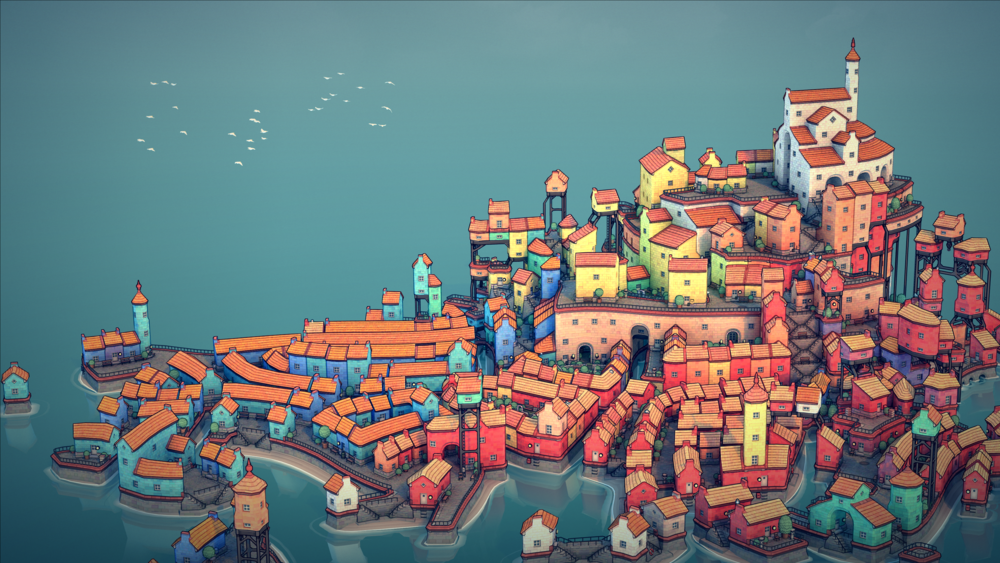
\includegraphics[width=\textwidth, height=0.3\textheight, keepaspectratio]{Images/Townscaper.png}
    \caption{Townscaper uses \acrshort{wfc} with player input to develop worlds \cite{townscaper}}
    \label{fig:townscaper}
\end{figure}

This dissertation applies the simple tiled implementation of \acrshort{wfc}. In simple tiled \acrshort{wfc}, a tile set with adjacency information is used by a constraint solver. This solver attempts to fill a grid of cells with tiles, taking into account their constraints. In the rest of this dissertation, this simple tiled implementation of \acrshort{wfc} is simply referred to as the \acrshort{wfc} algorithm.

% SIMPLE TILED WFC FIGURE
\begin{figure}[H]
    \centering
    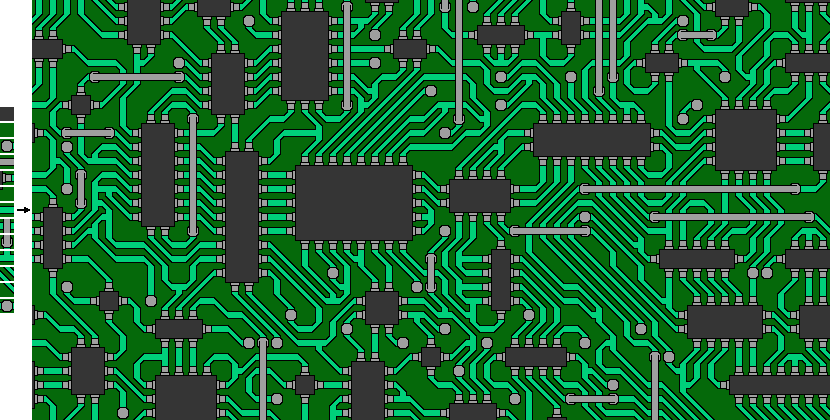
\includegraphics[width=\textwidth, height=0.3\textheight, keepaspectratio]{Images/circuit-1.png}
    \caption{Use of simple tiled \acrshort{wfc} to generate a circuit board graphic \cite{Gumin_Wave_Function_Collapse_2016}}
    \label{fig:WFCcircuit}
\end{figure}

% WFC has some issues: Lack of global constraints, overfitting and performance / scaling.
\acrshort{wfc}'s application is commonly limited by its lack of global constraints, overfitting and performance. Lack of global constraints can result in no inherent overall structure to the output, making it homogeneous. Use of complex tile sets can result in overfitting, reducing output variety. Complex tile sets and large grids also result in poor performance and increased failure rate.

% ESCHERESQUE FIGURE
\begin{figure}[H]
    \centering
    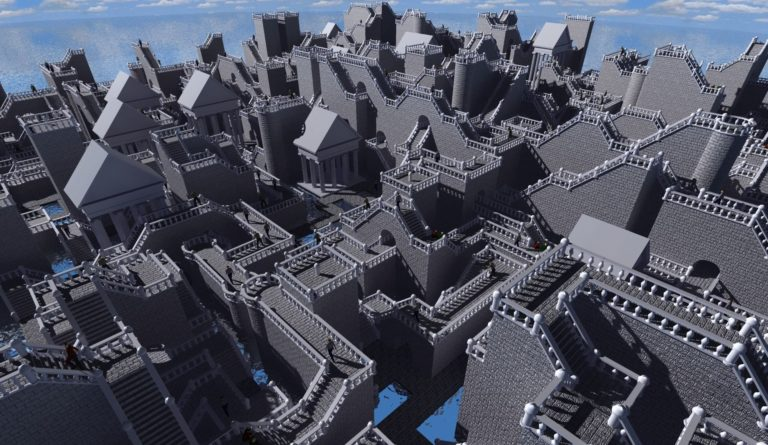
\includegraphics[width=\textwidth, height=0.3\textheight, keepaspectratio]{Images/escher_sample-768x445.jpg}
    \caption{A complex Escheresque tile set that relies on modifying in blocks \cite{model_synthesis_diss}}
    \label{fig:escheresque}
\end{figure}

% Solving these problems is often done in an ad hoc game-specific way that fails to exploit techniques from constraint programming literature.
These issues are rarely addressed directly in implementations. Instead, they are worked around in an ad hoc, game-specific way that fails to exploit constraint programming techniques.

% This work draws an explicit connection between WFC and MAC3 and then presents an implementation in those terms.
Presentation of \acrshort{wfc} online often fails to acknowledge underlying constraint solving principles used by \acrshort{wfc}. Instead, alternative wording is used, which can make forming a deep understanding of the topic challenging. This dissertation draws an explicit connection between \acrshort{wfc} and the \acrfull{mac3} algorithm, presenting an implementation in those terms.

% It also presents:
% An implementation of an extension of WFC that scales world generation infinitely.
% An interface integrated into the Unity game engine for designers to use WFC on their own tilesets.
% A game that utilises the presented techniques.
This dissertation's \acrshort{wfc} implementation is extended using the \acrfull{imib} algorithm, which addresses the challenge of extending \acrshort{wfc} to an infinite space. Furthermore, an interface integrated into the Unity game engine for designers to use \acrshort{wfc} on their own tilesets is included and a simple game created as example.

% IMIB FIGURE
\begin{figure}[H]
    \centering
    \subfigure[After layer 1 has been generated]{
        
\includegraphics[width=0.475\textwidth, height=0.35\textheight, keepaspectratio]{Images/IMIB3.png}
        \label{fig:imib3}
    }
    \hfill
    \subfigure[Preparing layer 2 with overlap into layer 1]{
        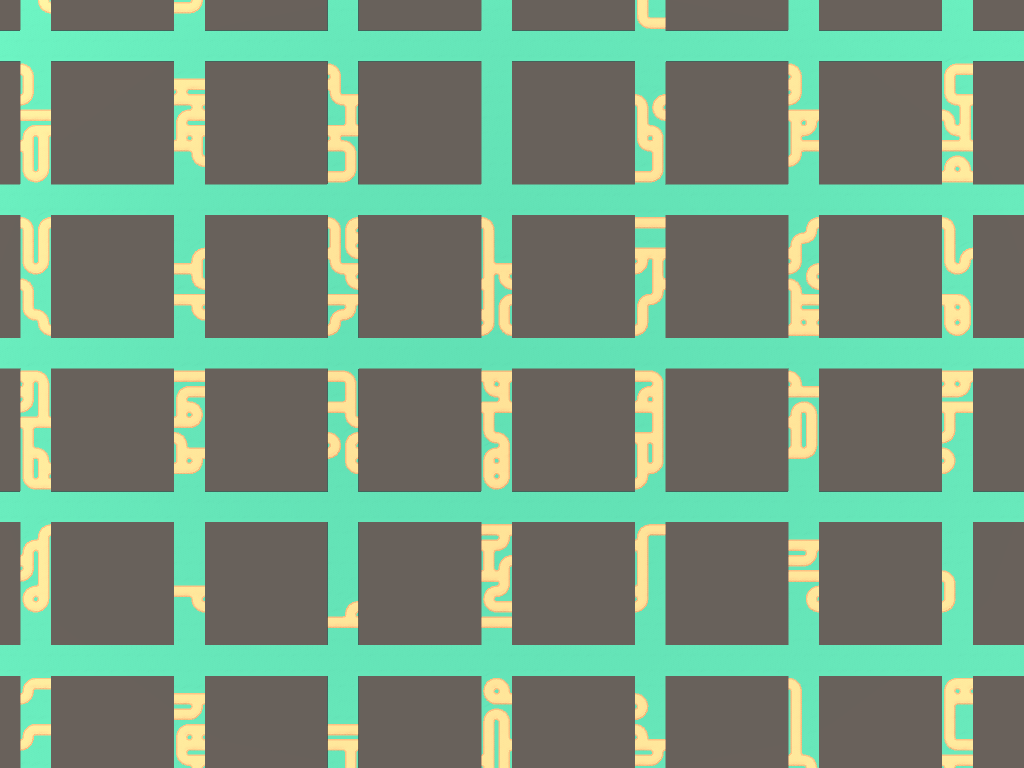
\includegraphics[width=0.475\textwidth, height=0.35\textheight, keepaspectratio]{Images/IMIB4.png}
        \label{fig:imib4}
    }

    \vspace{\baselineskip} % add some vertical space between the rows

    \subfigure[After layers 1 and 2 have been generated]{
        
\includegraphics[width=0.475\textwidth, height=0.35\textheight, keepaspectratio]{Images/IMIB5.png}
        \label{fig:imib5}
    }
    \hfill
    \subfigure[After all layers have been generated]{
        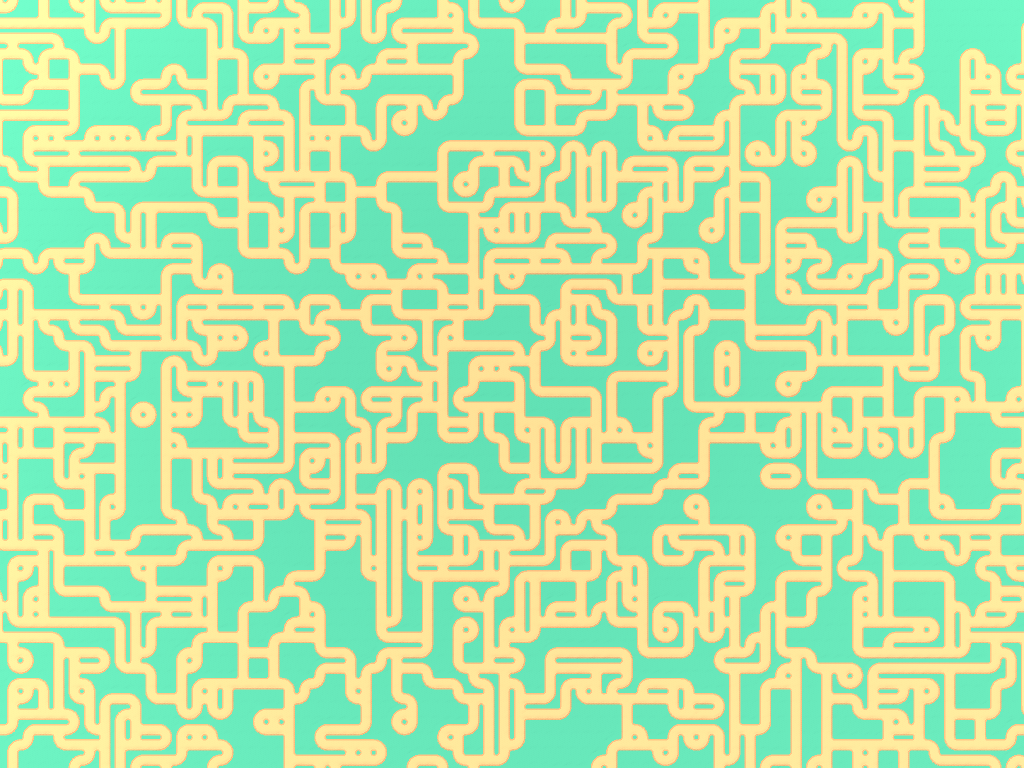
\includegraphics[width=0.475\textwidth, height=0.35\textheight, keepaspectratio]{Images/IMIB9.png}
        \label{fig:imib9}
    }
    \caption{A glimpse into the \acrshort{imib} pipeline. Each layer defines a small part of each chunk to run \acrshort{wfc} in. By clearing and running four overlapping layers, a full grid is generated. \cite{Infinite_Modifying_In_Blocks}}
    \label{fig:imib}
\end{figure}

%%%%% OLD INTRODUCTION
% Introduction to the project. Giving background on the areas covered (matching literature review).
%Wave Function Collapse (WFC) is a novel Procedural Content Generation (PCG) technique that has found significant use in video games \cite{Gumin_Wave_Function_Collapse_2016}. WFC can be described as a family of algorithms that enable generation of large game worlds from limited input through the application of constraint programming principles \cite{WFC_ConstraintSolving_and_ML}. This paper applies the simple tiled implementation of WFC, which uses a tile set with adjacency information on how to fit each tile together. The Maintaining Arc Consistency (MAC3) algorithm is then applied to a grid of cells to find a combination of tiles that satisfies adjacency constraints. MAC3 uses concepts of arcs and arc consistency to ensure constraints are satisfied at the start of generation and then maintain satisfaction as tiles to place are chosen. In the rest of the paper, this simple tiled implementation of WFC is simply referred to as the WFC algorithm.

% SIMPLE TILED WFC FIGURE
%\begin{figure}[H]
%\centering
%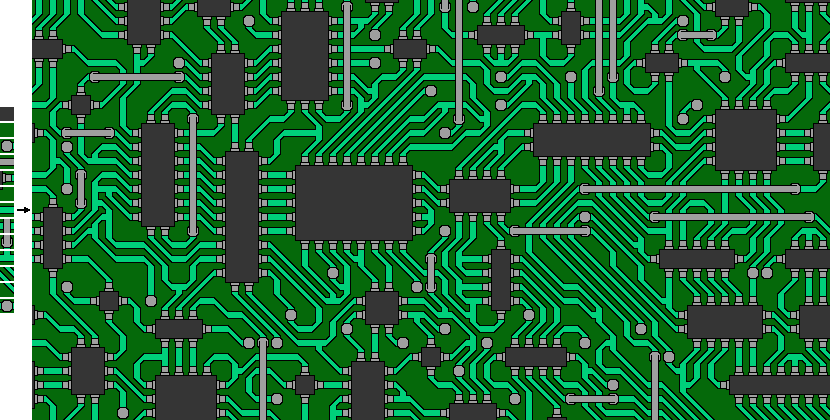
\includegraphics[width=\textwidth, height=0.3\textheight, keepaspectratio]{Images/circuit-1.png}
%\caption{Use of simple tiled WFC to generate a circuit board graphic %\cite{Gumin_Wave_Function_Collapse_2016}}
%\label{fig:WFCcircuit}
%\end{figure}

% Typical practices.
%WFC is often used as a `black box' in a workflow without being altered \cite{WFC_In_The_Wild}. It has had specialised applications in larger workflows in games such as Caves of Qud \cite{cavesofqud}, Townscaper \cite{townscaper} and Bad North \cite{badnorth}. This works around issues like its lack of global constraints, overfitting and performance.

% TOWNSCAPER FIGURE

% Issues to improve upon and how the issues have been addressed.
%One issue with WFC is that complex tile sets and large output areas can present a huge challenge to the constraint solver. In this situation, the solver has a high chance of failing to find a solution without backtracking. The amount of backtracking required can quickly scale with complexity, making just backtracking an infeasible solution. One way that input complexity and output size limitation have been addressed is through the modifying in blocks technique. This was first applied in Model Synthesis, an algorithm that served as inspiration for WFC \cite{model_synthesis}. This breaks the problem down into overlapping blocks that are simpler to evaluate. This generates similar output with a higher chance of success at the cost of additional generation from block overlap.

% ESCHERESQUE FIGURE

% Remaining issues
%One remaining issue is that this generation is on a finite grid. Infinite modifying in blocks addresses this by splitting the world into layers that can be deterministically generated in parallel to create chunks \cite{Infinite_Modifying_In_Blocks}. Parts of this pipeline can be seen in Figure \ref{fig:imib} and are explained in detail in Section \ref{sec:IMIB}. In addition to this, efficient handling of chunk loading and unloading is required. One novel optimisation included the direct calculation of new chunks to load relative to old chunks.

% IMIB FIGURE

% What this projects wants to address in the areas of focus.

% Address how the areas link together.
% Overall aim of the project.
% List of aims as in requirements specification?
% Which aims were achieved and how? Don't have too much detail. This is for the evaluation.